\chapter{State of the Art in Factoid Question Answering}
\label{ch:survey}

The research in Question Answering has been proceeding in several,
largely independent, directions.  The main division is between QA
on structured knowledge bases (typically graph databases like the
semantic web)


\section{Structured Data QA}
\label{sec:structured}

When answering questions on structured data, we can further
consider either helping users access relational databases (Natural Language Interface to Databases; NLIDB)
or finding matching relationships in the linked data graph of semantic web (Ontology-based Question Answering; QALD).

We are not aware of any significant recent work in the NLIDB domain
that would be based on well defined, published dataset and rigorously
evaluate results --- most research concerns building auxiliary systems
that augment human database experts. \citep{BergamaschiKeymantic, BlunschiSODA}
We do not consider this branch of research further.

QALD is much richer field of research, with yearly challenges \citep{QALD} and
popular reference datasets Free917 \citep{Free917} and WebQuestions \citep{WebQuestions}.
The reference knowledge base is typically Freebesa \citep{Freebase},
which holds a large amount of open domain real-world facts.%
\footnote{Freebase has been phased out into legacy state at this point.
	WikiData is set to replace it, but the migration of knowledge
	is still ongoing.}
QALD is one of the benchmarks for the semantic parsing task, aiming
to semantically parse a naturally phrased question into a structured
expression representing a graph query. \citep{SPBerant2014Paraphrase, Semantic2014Bordes}

\citep{Semantic2014Bordes} proposed a classification of QALD methods
that we will adopt, outlining two general strategies:

\begin{quote}
\textbf{Information
Retrieval (IR)} systems first retrieve a broad set of candidate answers by querying
the search API of KBs with a transformation of the question into a valid
query and then use fine-grained detection heuristics to identify the exact answer
(Kolomiyets survey 2011, Unger et al. 2012 templates, \citep{TreeFreebase2014Yao} TODO).
On the other hand, \textbf{Semantic Parsing (SP)} methods focus on the correct
interpretation of the meaning of a question by a semantic parsing system. A
correct interpretation converts a question into the exact database query that
returns the correct answer. \citep{Semantic2013Berant, SPBerant2014Paraphrase, OQA}
\end{quote}

These two strategies have been also compared in detail in \cite{FreebaseQA2014Yao}
and appear roughly comparable in accuracy.

\subsection{Dataset and Evaluation}

The most popular question dataset is WebQuestions \citep{WebQuestions},
which contains 3778 training and 2032 testing questions generated
automatically by a combination of Google Suggest API and Freebase
and with the gold standard answers manually produced by Amazon Mechanical Turk workers.%
\footnote{The gold standard has noise level of about $5\%$ questions,
	based on manual error analysis of a Google QA test on a movies sub-sample.}
Answers are always Freebase entities --- never relations themselves,
literals like numerical quantities, metadata like counts, or whole sentences.
Sometimes, the correct answers are lists of entities.
Extra measurements on customized versions of TREC (see below) and WikiQuestions
datasets are also sometimes published.

There is no complete consensus on benchmarking metrics in this task,
owing to different strategies in the systems.  Most generate an ordered
list of answers, and
\cite{Fader2013Paraphrase} uses \textit{answer precision} as the proportion of returned answers that are true,
while \textit{question recall} would be the proportion of questions that are correctly answered;
however,
\cite{TreeFreebase2014Yao} defines \textit{answer recall} more naturally
as a proportion of true answers that were returned.
On the other hand,
\cite{Semantic2013Berant}
almost always generates just a single
answer (or ``precise'' list, in case of a list question)
for every question and thus measures just the \textit{accuracy}.
The most common measure shared by most papers is F$_1$
(with recall as a proportion of correct answers found).
However, even this measure comes in two variations:
\textit{F$_1$ (Berant)} is average of precision/recall harmonic means per question,%
\footnote{This is about the same as the accuracy in \cite{Semantic2013Berant} style systems.
When comparing using this measure in ranked-answers systems,
a single answer is often forced even if none would be produced for the question otherwise. \citep{TreeFreebase2014Yao}}
while \textit{F$_1$ (Yao)} is harmonic mean of answer precision and recall computed across all questions.

A caveat of these measures is that they put emphasis on the complete
set of returned answers, rather than just focusing on the top of
the ranked list.  Thus, in addition IR-style measures are also often
used.
\cite{Semantic2014Bordes} uses
\textit{precision@1} as the proportion of questions that have a correct answer ranked first.
\textit{MRR} (Mean Reciprocial Rank) can capture the average rank the correct answer appears at,
while \textit{MAP} (Mean Average Precision) is not as intuitively interpretable, but generalizes
even to a scenario with multiple expected correct answers.

\subsection{Information Retrieval Approach}

\textbf{Information Extraction over Structured Data: Question Answering with Freebase (Jacana Freebase)} \citep{TreeFreebase2014Yao}
	--- TODO.
		Open source.

\textbf{Lean Question Answering over Freebase from Scratch (kitt.ai)} \citep{LeanFreebaseYao}
	--- simple fuzzy string matching to identify Freebase concepts,
		bag-of-words logistic regression to identify relations.
		WebQuestions F1 Berant 44.3\%, F1 Yao 53.5\%.

\subsection{Semantic Parsing Approach}

\textbf{Open Question Answering Over Curated and Extracted Knowledge Bases (OQA)} \citep{OQA}
	--- paraphrase (mined operators) $\to$ parse (templates) $\to$ rewrite (mined operators) $\to$ execute (ensemble of KBs).
	Novel machine learning for inference and answer scoring with hidden variables.
	Datasets public, open source.
	WebQuestions F1 35\%, TREC F1 29\%, WikiAnswers F1 8\%.

\textbf{(Paralex)} \citep{Fader2013Paraphrase}

\textbf{(SEMPRE)} \citep{SPBerant2014Paraphrase}





\section{Unstructured Data QA}
\label{sec:unstructured}

When dealing with question answering on top of unstructured data,
two research directions exist: aside of generating a crisp answer,
\textit{Answer Sentence Selection} is a popular sub-task%
\footnote{\url{http://aclweb.org/aclwiki/index.php?title=Question_Answering_\%28State_of_the_art\%29}}
where instead of the answer, just an appropriate answer-bearing passage
is to be returned to the user.

\subsection{Dataset and Evaluation}

The main benchmarked dataset is a collection of TREC competition datasets
from the turn of the century,%
\footnote{\url{http://trec.nist.gov/data/qamain.html}}
on top of the AQUAINT newswire corpus;
as gold standard,
regular expressions matching the answers judged correct were provided.
Compared to e.g. WebQuestions + Freebase, the TREC questions
are more realistic in open domain user QA setting --- they are diverse
in answer type and level of detail and of quite varying difficulty.
On the other hand, naive usage of this dataset hits a few major issues:

\begin{itemize}
	\item The AQUAINT corpus is not freely available, and some of the questions are dependent on that time period (like population numbers or persons occupying public positions) or are highly specific (referring particular individual news articles).
	\item Regular expressions are limited when matching alternative spellings or name abbreviations, and almost break down when matching entities such as dates or dimensional quantities (possibly using different units).
	\item There are no well-defined train/test splits, datasets for individual years significantly vary in character, and even the years included in summary TREC datasets differ.
\end{itemize}

Therefore, measurements on TREC are very difficult to compare.  Many papers
declare that they subsampled the dataset in arbitrary ways or judged correct
answers manually.  We attempt to rectify this situation for future comparisons
in Sec.~\ref{sec:expsetup}.

The typical IR metrics of \textit{MRR} and \textit{MAP} are commonly
used, as well as \textit{precision}, \textit{recall} and \textit{F$_1$}.
Consider a question answered correctly if the top-ranked answer is correct:
then, precision is the proportion of correctly answered questions to all
answered questions,%
\footnote{Except some outliers; \cite{Ephyra2006} uses the ``precision'' term
	to denote AP recall.}
while recall would be the proportion of correctly answered questions to all
questions altogether --- this definition is shared by
e.g.\ \cite{TreeEdit2013Yao} and \cite{QuASE}.
\cite{WatsonOverview} uses \textit{precision@75} to denote a proportion
of questions that are answered correctly when attempting to answer 75\% of questions.

TREC competitions used MRR \citep{TREC8,TREC9,TREC10},
confidence-weighted score $1/Q \sum_{i=1}^Q \textrm{precision-at-$i$} / i$ \citep{TREC11},
as well as requiring only single answer returned and computing simple accuracy \citep{TREC12}.

Many unstructured QA systems are primarily IR machines that follow
an overproduce-and-choose answer production strategy.  To measure
the answer production performance, \cite{WatsonIR} uses \textit{candidate binary recall},
that is the number of questions where a correct answer has been generated as a candidate
for scoring;
we also use this measure, but prefer the term \textit{answer production (AP) recall}.


\subsection{Answer Sentence Selection}
\label{sec:anssentsel}

Binary classification or ranking problem.
TODO TREC-based dataset by Wang et al.
MAP and MRR reported.

\textbf{(Jacana)} \citep{TreeEdit2013Yao}

\textbf{Deep Learning for Answer Sentence Selection} \citep{Yu2014Deep}
	--- given vector embeddings $\mathbf{q}, \mathbf{a}$, estimate
	$P(rel|q,a) = \sigma(\mathbf{q}^T \mathbf{M}\, \mathbf{a} + b)$
	i.e.\ train a model with parameters $\mathbf{M}, b$ that
	generates a likely question embedding using $\mathbf{M}\, \mathbf{a}$
	and then using dot-product measures its distance to the posed question.
	Cross entropy over all QA pairs is used as the loss function for training.
	Off-the-shelf $d=50$ distributed representations by Collobert and Weston 2008
	are used as word embeddings.
	To generate compositional embeddings,
	a simple unigram model that averages the embeddings is the baseline;
	as a small ($\Delta 0.02$) improvement, bigram model is proposed that uses a CNN
	on the sentence with a bigram convolutional layer and an average-pooling layer.
	To deal with numbers and proper nouns, a token co-occurrence counter
	feature is also used; the learnt method gives $\Delta 0.125$ against this baseline.
	TREC MAP 0.7113, MRR 0.7846.

\subsection{Precise Answer Production}

TREC benchmark.  Curated TREC.  WebQuestions also possible(?).

\textbf{(DeepQA IBM Watson)} \citep{WatsonOverview}

\textbf{(Jacana)} \citep{TreeEdit2013Yao} \citep{TreeEditIR2013Yao}
is a promising set of loosely coupled QA-related methods
and algorithms, focused on machine learning of textual entailment.  It is
not meant to be a full QA framework and using it as an end-to-end pipeline
is not straightforward, but integration of the Jacana implementation as
modules in YodaQA is our long-term plan.

\textbf{Web-based Question Answering: Revisiting AskMSR (AskMSR+)}

\textbf{Open Domain Question Answering via Semantic Enrichment (QuASE)} \citep{QuASE}
	--- web-based QA system that links snippet pieces to Freebase entities
	\textit{(entity linking)} to generate extra features for answers.
	One feature is the cosine similarity of word
	vectors corresponding to question (and web-fetched question support)
	and answer's textual propreties (like \textit{description}) in Freebase
	(N.B. word frequency vectors, not embeddings!).
	Another feature is probabilistic type matching by bag of words Bayes model
	with Perplexity.  Generative mixture model with Dirichlet priors is used
	for answer scoring.  Compared to naive web search baseline, TREC F1
	improvement was 3.5\%.  (Absolute numbers not comparable due to
	sub-sampling and re-evaluation.)

\textbf{YodaQA: A Modular Question Answering System Pipeline} \citep{YodaQAPoster2015}

The classic QA system \textbf{OpenEphyra} \citep{Ephyra2006}
operates on the basis of fixed question categories with hand-crafted rules,
and puts emphasis on querying web search engines.
The \textbf{OAQA} initiative \citep{OAQATowards} has developed a basic QA framework,
but does not provide an end-to-end pipeline and its usage of UIMA has
in our opinion severe design limitations (see below).
The \textbf{WatsonSim} system \citep{WatsonSim} has begun developing independently
during the course of our own work and it works on Jeopardy! statements rather
than questions.

\textbf{MemNets} though I still think it's a toy task in QA context.

\section{Auxiliary Tasks in QA}

\subsection{Question Classification}

In datasets which ask mostly uniform types of answers (e.g. WebQuestions,
where the answer is always an entity), it may be possible to use the same
set of features to produce and score answers across all questions.
However, e.g.\ in the TREC dataset, types of answers vary widely and
different strategies might be appropriate (even if they are to be machine
learned rather than hardcoded, as was common in the early systems).

One approach is to classify an answer to a fixed set of categories.
A two-level (coarse, fine) taxonomy based on the TREC set of questions and a labelled dataset%
\footnote{\url{http://cogcomp.cs.illinois.edu/Data/QA/QC/}}
was introduced by \textbf{Learning question classifiers} \citep{QCLearning}.
They set a baseline of coarse $P_1=91.0\%$, fine $P_1=84.2\%$.

This sentence classification problem has been one of the standard benchmarks
for semantic NLP tasks:
\begin{itemize}
	\item SVM$_S$ (Silva et al., 2011) TODO coarse $P_1=95.0\%$
	\item DCNN \citep{QtcDCNN} TODO coarse $P_1=93.0\%$
	\item CNN \citep{CNNSentClass} coarse $P_1=93.6\%$
	\item Skip-Thought Vectors \citep{SkipThought} coarse $P_1=92.2\%$ (but unsupervised)
	\item Self-Adaptive Hierarchical Sentence Model \citep{AdaSent} (AdaSent) coarse $P_1=92.6\%$
	\item TODO more papers; \citep{AdaSent} has some references; separate embedding and classical?, supervised and unsupervised; even primitive baseline is something like $85\%$
\end{itemize}

A different approach that was introduced by IBM Watson DeepQA \citep{WatsonTyCor}
associates the question with a Lexical Answer Type (LAT) which is
an arbitrary English word that would describe the answer concept
(e.g. ``inventor'' or ``length'').

\subsection{Entity Linking}
\label{sec:entitylink}

When a question is analyzed, one of the main tasks is typically recognition
of entity mentions in the question text.  The system should process all
varions of ``When did John F. Kennedy die?'', ``When did JFK die?'',
``When did Kennedy die?'' and ``Wehn did Kenndey die?''.  An intelligent
system needs to correctly link entities using aliases or ambiguous
references and stay resistant to typos.

\textbf{Improving Entity Linking using Surface Form Refinement}

\url{http://nlp.cs.rpi.edu/kbp/2014/elreading.html}

TODO \dots

\subsection{Answers by Paraphrasing}

Many questions ask essentially for a paraphrase of the term under
question --- for example, the question ``Who is a plumber?'' wants
to find out a description of \textit{plumber} without using these
words, while ``What is the capital of Christians?'' may seek the
paraphrase of \textit{capital of Christians}, aside of database lookups.

\textbf{Learning to Understand Phrases by Embedding the Dictionary (DefGen)} \citep{DefGen}
	--- reverse dictionary and QA on crossword puzzles using word2vec
	with composing via RNN or an averaging baseline, embeddings of
	concepts are pre-trained from wikipedia intros and wordnet definitions.

\subsection{Cloze-style Questions}

In the Cloze procedure scenario \citep{Cloze},
we consider a $(context, query)$ pair where the query
sentence is entailed by the context, but a single entity name in the query
is missing (e.g.\ in a context detailing an incident of the well-known personality
\textit{Jeremy Clarkson}, we are to find $X$ for the query
\textit{Producer X will not press charges against Jeremy Clarkson, his lawyer says.}).

\textbf{Teaching Machines to Read and Comprehend} \citep{ReadAndComprehend}
	--- an attention-based model that produces vector embeddings of $(document, query)$
	pairs and uses a weight matrix to judge probability of a particular
	word being the answer based on the composite pair embedding;
	the paper is not clear on the particulars, unfortunately.
	Three composite vector embedding models are considered,
	based on bi-directional LSTM and convolution-ish architectures.




\section{Hybrid QA Systems}

Full-scale end-to-end systems combining structured and unstructured approaches.

\textbf{(DeepQA IBM Watson)} \citep{WatsonOverview}

\textbf{YodaQA: A Modular Question Answering System Pipeline} \citep{YodaQAPoster2015}

\textbf{OpenQA} \citep{OpenQA} is a recently introduced end-to-end QA pipeline platform
also developed independently during the course of our work, and shares our
goal of a common research platform in the field.  However, the approach
is very different, as OpenQA is more of a portfolio-style engine with
mostly independent pipelines which have their candidate answers combined,
while YodaQA emphasizes modularity on the pipeline stage level,
with e.g.\ all answer producers sharing a common answer analysis stage.





\section{Non-Factoid QA}
\label{sec:nonfactoid}

TODO very short overview.  The MemNN task.  Text entailment.





\section{Vector Embeddings of Words}
\label{sec:embeddings}

TODO rewrite, expand.

Recent progress in NLP has been marked mainly by the proliferation of
so-called \textit{vector embeddings}, the most popular being called
\textit{word2vec}.  This approach stems from the so-called \textit{distributional semantics}
hypothesis, which posits that we can derive meanings of words purely
from the context they tend to appear in.  Therefore, each word is
associated with a list of $n$ real numbers (i.e.\ coordinates of
an $n$-dimensional vector) and these numbers are derived automatically
just from the context the words appear in.%
\footnote{The \textit{word2vec} method uses an idea called \textit{multi-task learning}
	which may be useful for us as well --- we try to learn
	some easy-to-specify task and then we re-use the same model to
	solve some much harder problems.  Here, the $n$ real numbers
	come out from training a classifier that predicts the most likely
	next words to come given a context of (say, 100) preceding words;
	this so-called \textit{language model} task is useful e.g.\ in
	speech recognition or OCR.}
The interesting property is that the automatically assigned numbers
exhibit semantic properties in how they relate between words.
For example, if we do arithmetics on these word vectors and try
to compute e.g.\ $king + (woman - man)$, the nearest vector we reach
is $queen$, i.e.\ the gender transition is represented by an arrow
in our vector space (Fig.~\ref{fig:w2vg}).
Fig.~\ref{fig:w2ver} shows how relationships between adjectives are represented
while Fig.~\ref{fig:w2vc} shows mappings between coordinates of countries
and their capitals.  Let us emphasize again that these coordinates were
determined purely based on the context of the words (in Wikipedia or
millions of news articles); the system did not have any extra information
or databases available.

\begin{figure}[ht]
	\centering
	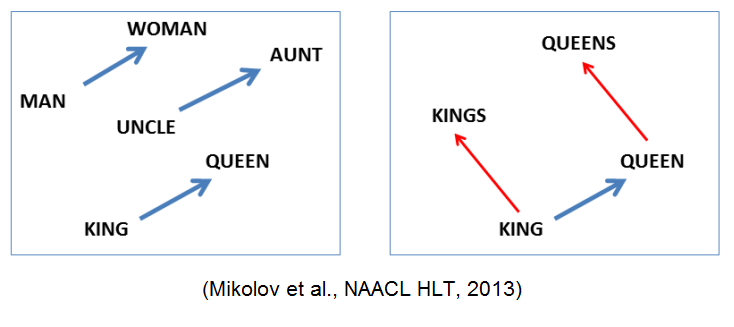
\includegraphics[width=10cm]{kingqueen.png}
	\caption{Semantic relationships between words as arrows in the vector space. \citep{WordVecLingReg}}
	\label{fig:w2vg}
\end{figure}

\begin{figure}[p]
	\centering
	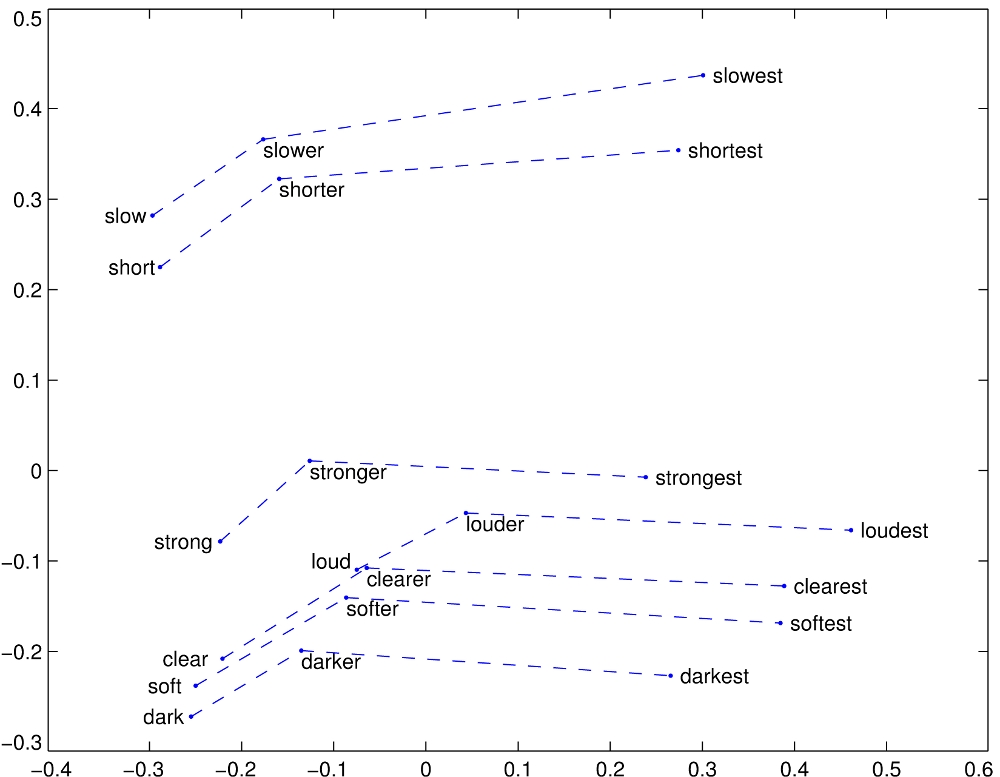
\includegraphics[width=10cm]{comparative_superlative.jpg}
	\caption{Semantic relationships between superlative adjectives as represented in the vector space.
		This is a 2D projection of the high-dimensional space that is designed to well preserve relative positions of the shown entities
		(so-called t-SNE 2D).
		\citep{Glove}}
	\label{fig:w2ver}
\end{figure}

\begin{figure}[p]
	\centering
	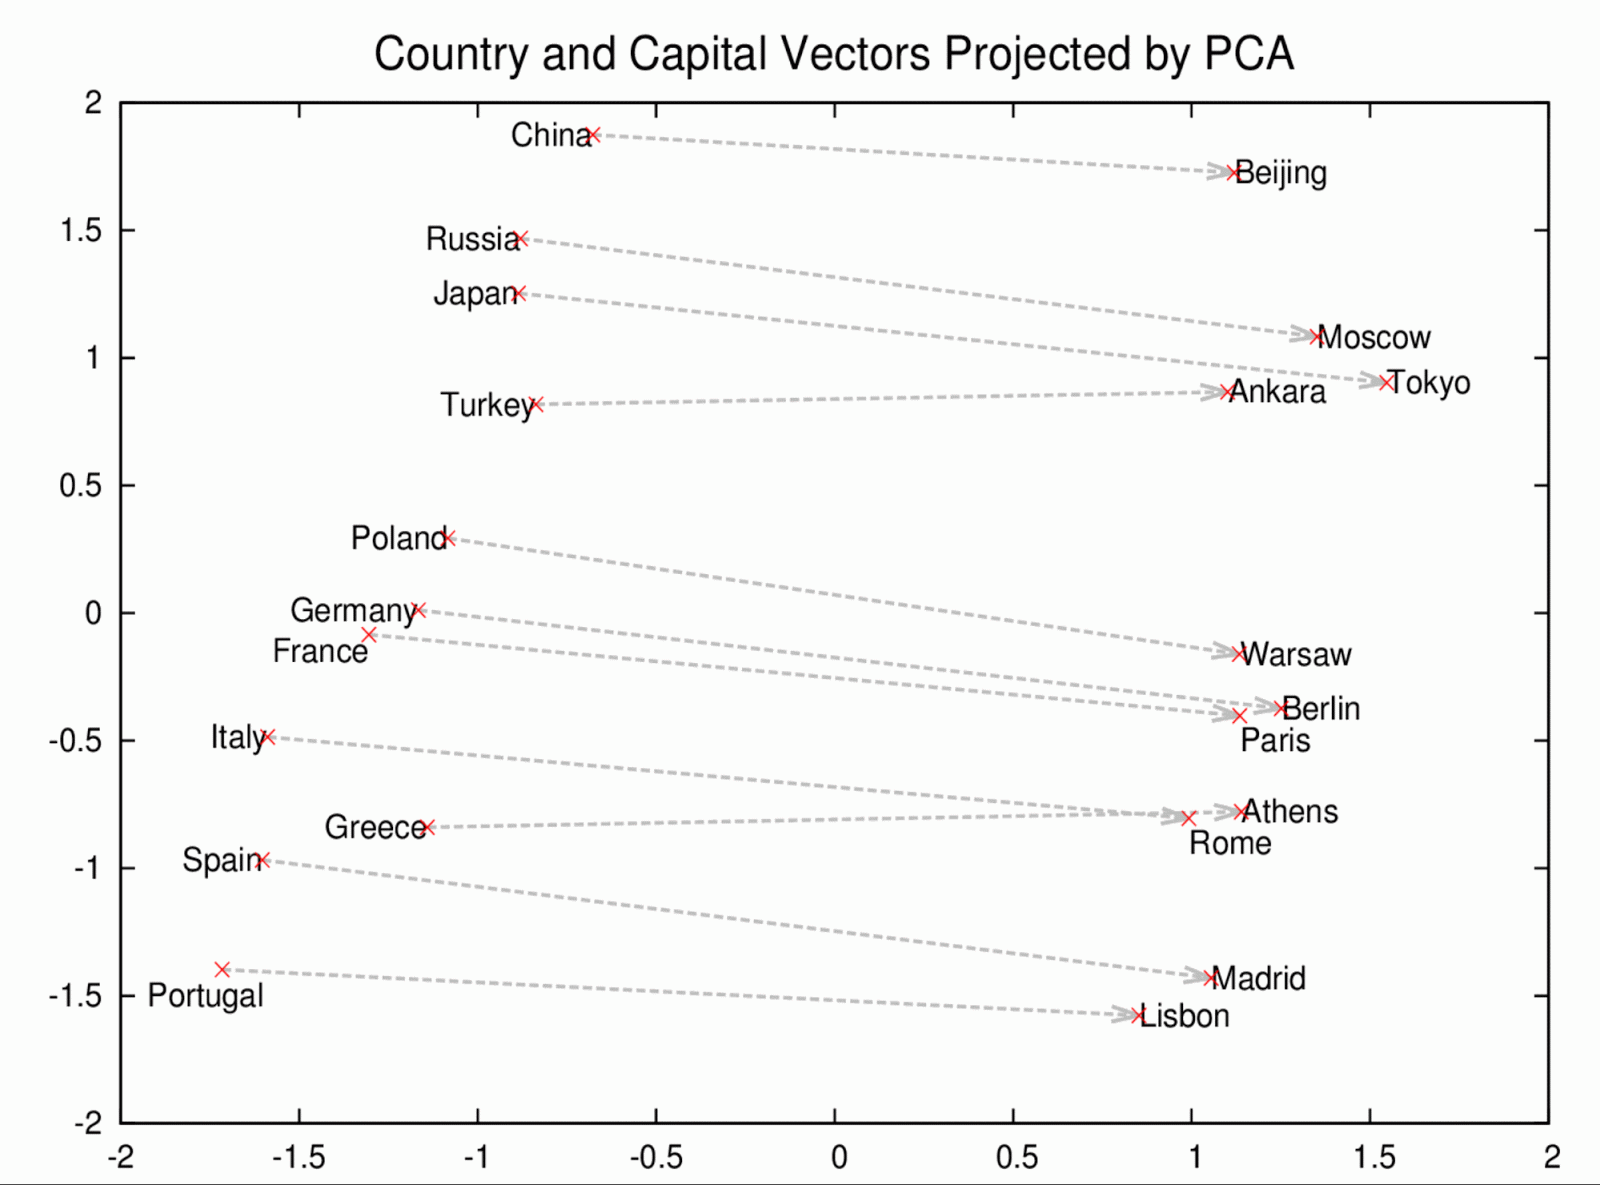
\includegraphics[width=11cm]{capitals.png}
	\caption{Mappings between countries and capitals, acquired entirely from the typical context of the respective words.
	This is again a 2D projection of the high-dimensional space, this time obtained by a PCA dimensionality reduction technique.
	\citep{DistReprComp}}
	\label{fig:w2vc}
\end{figure}

A lot of the current research focuses on the best ways to build up
vector representations of whole sentences and documents --- ranging
from simple averaging \citep{CNNSentClass,DefGen} (successful baselines)
to recurrent neural networks \citep{LISA,ShowAndTell}.
Many applications that rely on semantic understanding of word nuances
are popping up; this method became state-of-art for machine translation
\citep{LISA}, automatic image captioning \citep{ShowAndTell} and specific
types of question answering \citep{QANTA,DefGen,ReadAndComprehend}%
\footnote{The demo at \url{http://45.55.181.170/defgen/} is nice.}.
One open problem is efficient composition of vector embeddings for
common words with entities like numbers or proper names.
